\documentclass{beamer}
\usepackage[latin1]{inputenc}
\usepackage{hyperref}
\usetheme{Singapore}
\title[RUM 2]{RUM 2}
\bibliographystyle{unsrt}
\author{Mike DeLaurentis}
\institute{University of Pennsylvania}
\date{August 15, 2012}
\usepackage{listings}

\AtBeginSection[]
{
  \begin{frame}<beamer>
    \frametitle{Agenda}
    \tableofcontents[currentsection]
  \end{frame}
}


\begin{document}

\begin{frame}
\titlepage
\end{frame}

\begin{frame}{Agenda}
  \tableofcontents
\end{frame}

\begin{frame}{About me}
  \begin{itemize}
  \item Software engineering background
  \item Working at Penn since January
  \item Experience in a variety of languages (Perl, Java, Clojure (lisp), Python, Ruby)
  \end{itemize}
\end{frame}

\section{The RUM Pipeline}

\begin{frame}{About RUM}
  \begin{itemize}
  \item ``RUM is an alignment, junction calling, and feature quantification pipeline specifically designed for Illumina RNA-Seq data''
  \item Written by Gregory Grant (ggrant@grant.org)
  \item Runs on Linux / UNIX / Mac
  \item Can distribute work across multiple machines
  \item Written in Perl 5
  \end{itemize}
\end{frame}

\begin{frame}{The RUM Pipeline}
\begin{itemize}
  \item Align all reads against genome using Bowtie
  \item Align all reads against transcriptome using Bowtie
  \item Merge genome and transcriptome alignments and identify unmapped reads
  \item Align unmapped reads against genome using BLAT
  \item Merge Bowtie and Blat alignments
  \item Produce some output files based on merged results
\end{itemize}
\end{frame}

\begin{frame}{RUM output files}
  \begin{columns}
    \column{2.5in}
\begin{itemize}
  \item Files of unique and non-unique alignments
  \item All alignments in SAM format
  \item Coverage plots
  \item Feature quantifications
  \item Junction calls
  \item List of novel inferred internal exons
\end{itemize}
\column{2.5in}

\includegraphics[scale=0.4]{rumpouring2.png}
  \end{columns}

\end{frame}

\begin{frame}{Work distribution}
  \begin{columns}
    \column{2.5in}
    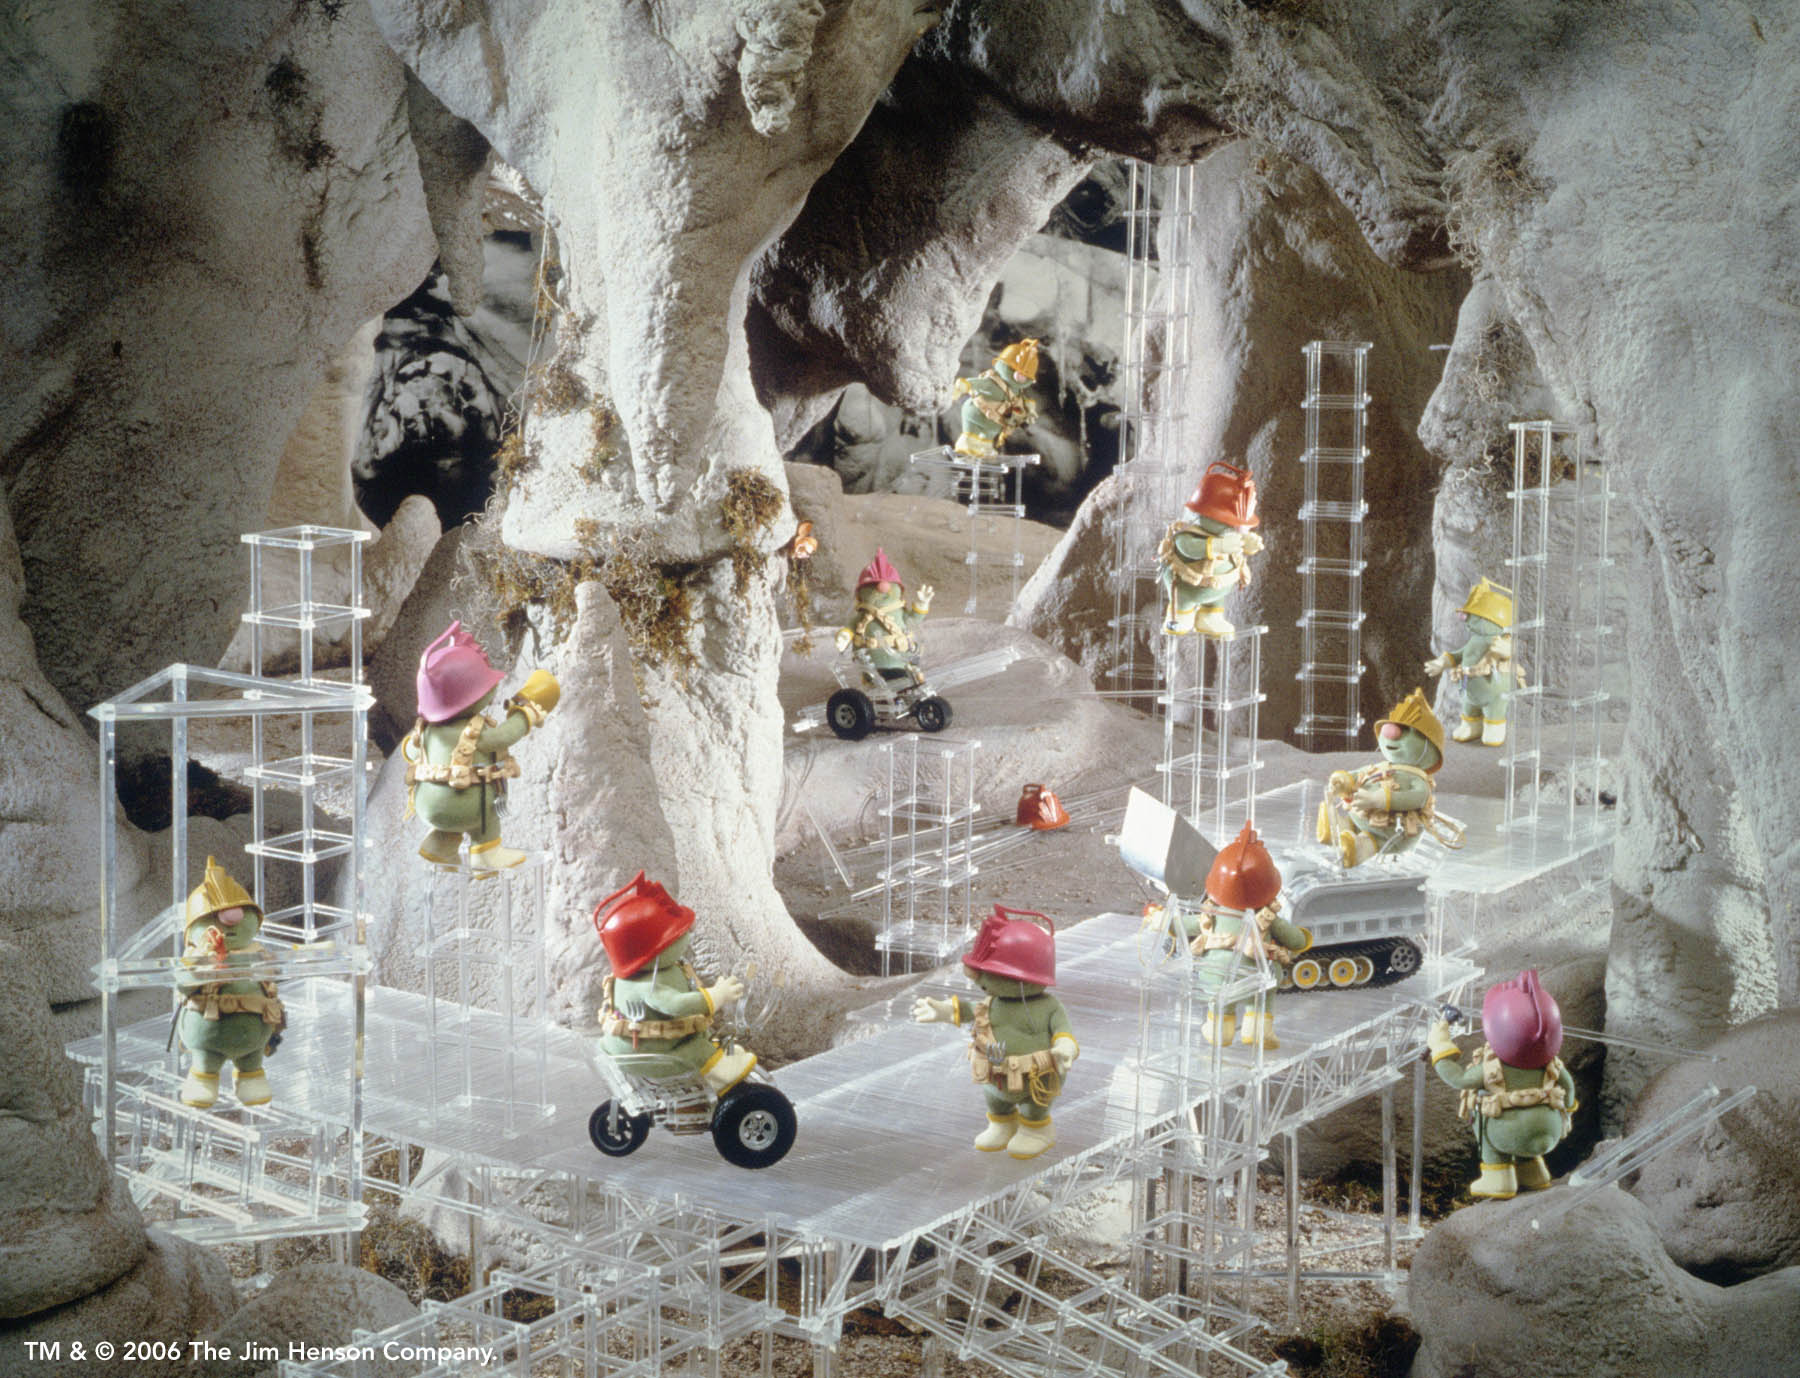
\includegraphics[scale=0.4]{doozers.jpg}    
    \column{2.5in}
    \begin{itemize}
    \item RUM can run alignment phase in parallel
    \item Splits input reads into N chunks
    \item Alignment for each chunk is independent of other chunks
    \item Results are merged together for coverage, quantification,
      junction calling
    \end{itemize}
  \end{columns}


\end{frame}

\section{Enhancements in RUM 2}

\begin{frame}{RUM 2 Features}
  \begin{itemize}
  \item Standard installation process
  \item New command-line interface
  \item Get status of running job
  \item Restart a job where it left off
  \item More reliable kill command
  \item Run a chunk or postprocessing by itself
  \item Relocatable indexes
  \item SAM file is closer to conforming to standard
  \end{itemize}
\end{frame}

\subsection{Installation}

\begin{frame}{Installation}
  \begin{itemize}
  \item Uses standard Perl Makefile.PL
  \item Should be familiar to system administrators
  \item Download tarball from \texttt{https://github.com/PGFI/rum/downloads}
  \item Run \texttt{perl Makefile.PL}
  \item Install indexes using \texttt{bin/rum\_indexes}
  \item That's it!
  \end{itemize}
\end{frame}

\subsection{Command-line interface}

\begin{frame}{Command-line interface}

  Usage is \texttt{rum\_runner ACTION [OPTIONS]} where action is one of:

  \begin{itemize}
  \item \texttt{align} - Run an alignment
  \item \texttt{status} - Check the status of a job
  \item \texttt{stop} - Stop a job (can be restarted later)
  \item \texttt{kill} - Stop a job and clean it up (to restart from scratch)
  \item \texttt{clean} - Remove output files for a job
  \item \texttt{help} - Get help
  \item \texttt{version} - Show version number
  \end{itemize}

\end{frame}


\begin{frame}[fragile]{rum\_runner align}
Use \texttt{rum\_runner align} to run an alignment:
\begin{verbatim}
rum_runner align \
  --output dir \
  --index  ~/rum_indexes/hg19 \
  --name   TestJob \
  --chunks 25 \
  ~/samples/forward.fq ~/samples/reverse.fq
\end{verbatim}
\end{frame}


\subsection{Job status}

\begin{frame}[fragile]{Job status}
  \begin{itemize}
  \item Use \texttt{rum\_runner status} to check on the status of a
    running job.
  \end{itemize}
  \tiny
\begin{verbatim}
Processing in 25 chunks
-----------------------
XXXXXXXXXXXXXXXXXXXXXXXXX Run bowtie on genome
XXXXXXXXXXXXXXXXXXXXXXXXX Parse genome Bowtie output
X XXX  XX XX XXXX  XXXXX  Run bowtie on transcriptome
X XXX  XX XX XXXX  XXXXX  Parse transcriptome Bowtie output
X XXX  XX XX XXXX  XXXXX  Merge unique mappers together
X XXX  XX XX XXXX  XXXXX  Merge non-unique mappers together
X XXX  XX XX XXXX  XXXXX  Make unmapped reads file for blat
X XXX  XX XX XXXX  XXXXX  Run blat on unmapped reads
X XXX  XX XX XXXX  XXXXX  Run mdust on unmapped reads
X XXX  XX XX XXXX  XXXXX  Parse blat output
X XXX  XX XX XXXX  XXXXX  Merge bowtie and blat results
X XX   XX XX  XXX   XXXX  Clean up RUM files
X XX   XX XX  XXX   XXXX  Produce RUM_Unique
X XX   XX XX  XXX   XXXX  Sort RUM_Unique by location
X X    XX XX  XXX   XXXX  Sort cleaned non-unique mappers by ID
X X    XX XX  XXX   XXXX  Remove duplicates from NU
X X    XX XX  XXX   XXXX  Create SAM file
X X    XX XX  XXX   XXXX  Create non-unique stats
X X    XX XX  XXX   XXXX  Sort RUM_NU
X X    XX XX  XXX   XXXX  Generate quants
...
\end{verbatim}
\end{frame}

\begin{frame}[fragile]{Job status}
\tiny
\begin{verbatim}
Postprocessing
--------------
  Merge RUM_NU files
  Make non-unique coverage
  Merge RUM_Unique files
  Compute mapping statistics
  Make unique coverage
  Finish mapping stats
  Merge SAM headers
  Concatenate SAM files
  Merge quants
  make_junctions
  Sort junctions (all, bed) by location
  Sort junctions (all, rum) by location
  Sort junctions (high-quality, bed) by location
  Get inferred internal exons
  Quantify novel exons

All the chunk error log files are empty. That's good.
Main error log file is empty. That's good.

RUM is running (job ids 815718, 815720).
\end{verbatim}
\end{frame}

\begin{frame}{Recovering from errors}
  \begin{columns}[c]
    \column{2.5in}
    
\includegraphics[scale=0.2]{success.jpg}
    \column{2.5in}
    \begin{itemize}

    \item Sometimes bad things happen

    \item RUM 2 allows easier recovery from infrastructure failures

    \item Running ``\texttt{rum\_runner align}'' again will restart a
      job from where it left off

    \item Can save \textit{a lot} of time when recovering from infrastructure failure

    \item Determines state of job by looking at which output files exist

    \end{itemize}

  \end{columns}
\end{frame}

\begin{frame}[fragile]{Killing a job}
\begin{itemize}
\item To stop a job and remove all of its output:
\begin{verbatim}
  rum_runner kill -o dir
\end{verbatim}
\item Useful if you've run a job with incorrect parameters and need to start over
\end{itemize}

\end{frame}

% http://tomboythatwearsmakeup.com/wp-content/uploads/2011/03/dz_fr_012-1.jpg

\section{Demo}

\section{Web resources}

\begin{frame}{Main Github page}
  \url{https://github.com/PGFI/rum}
  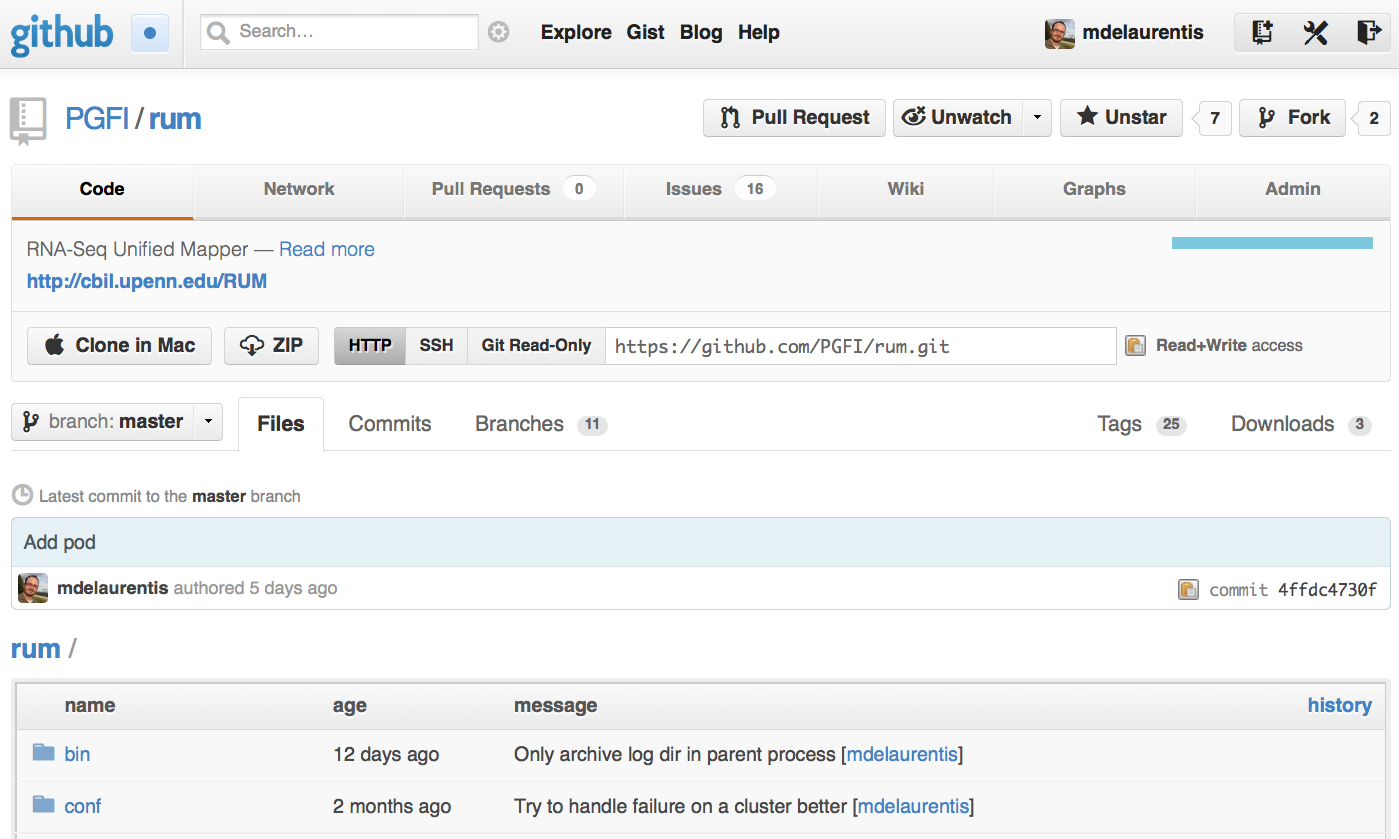
\includegraphics[scale=0.2]{github-main.png}
\end{frame}

\subsection{User guide}

\centering
\begin{frame}{User guide}
  \url{https://github.com/PGFI/rum/wiki}
  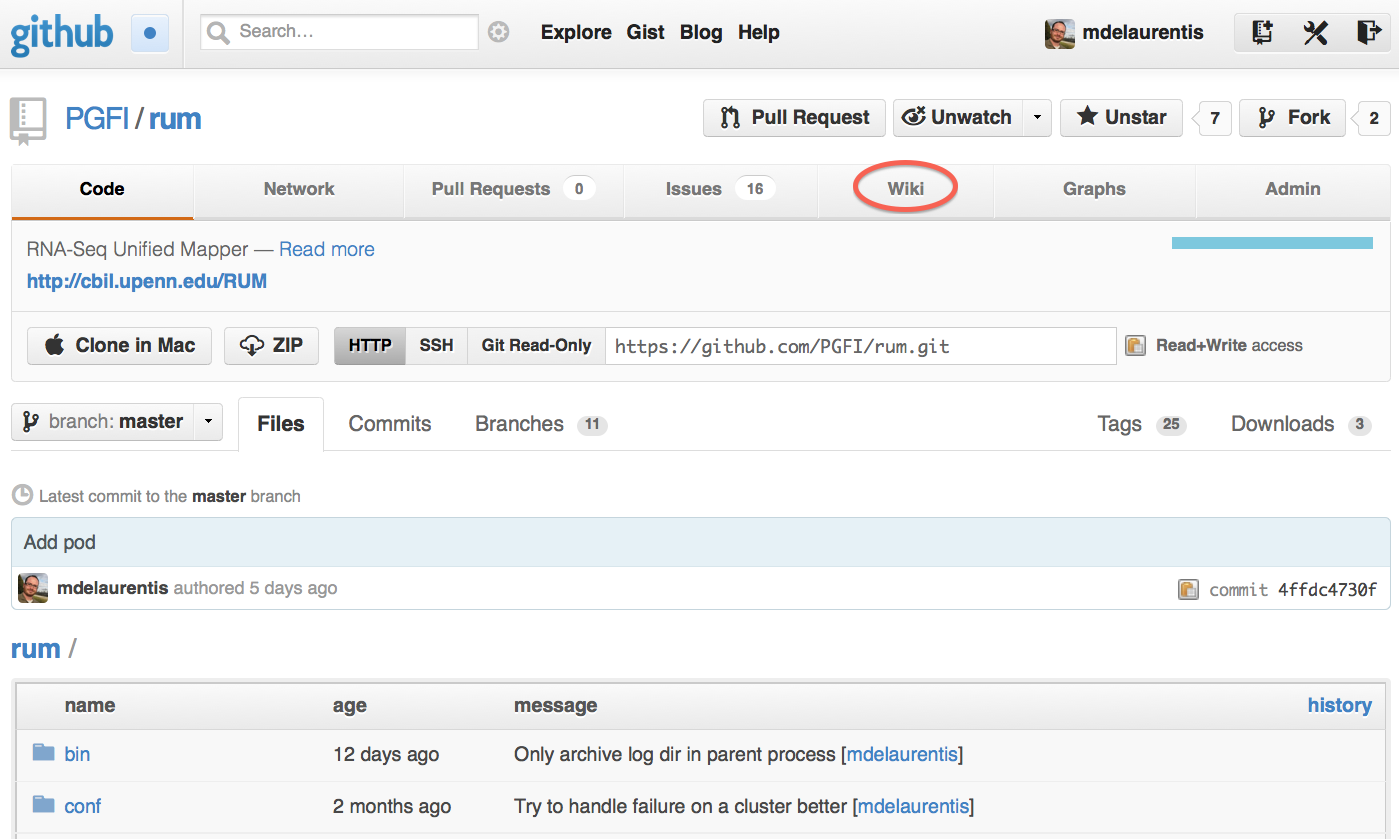
\includegraphics[scale=0.2]{github-main-wiki.png}
\end{frame}

\centering
\begin{frame}{User guide}
  \url{https://github.com/PGFI/rum/wiki}
  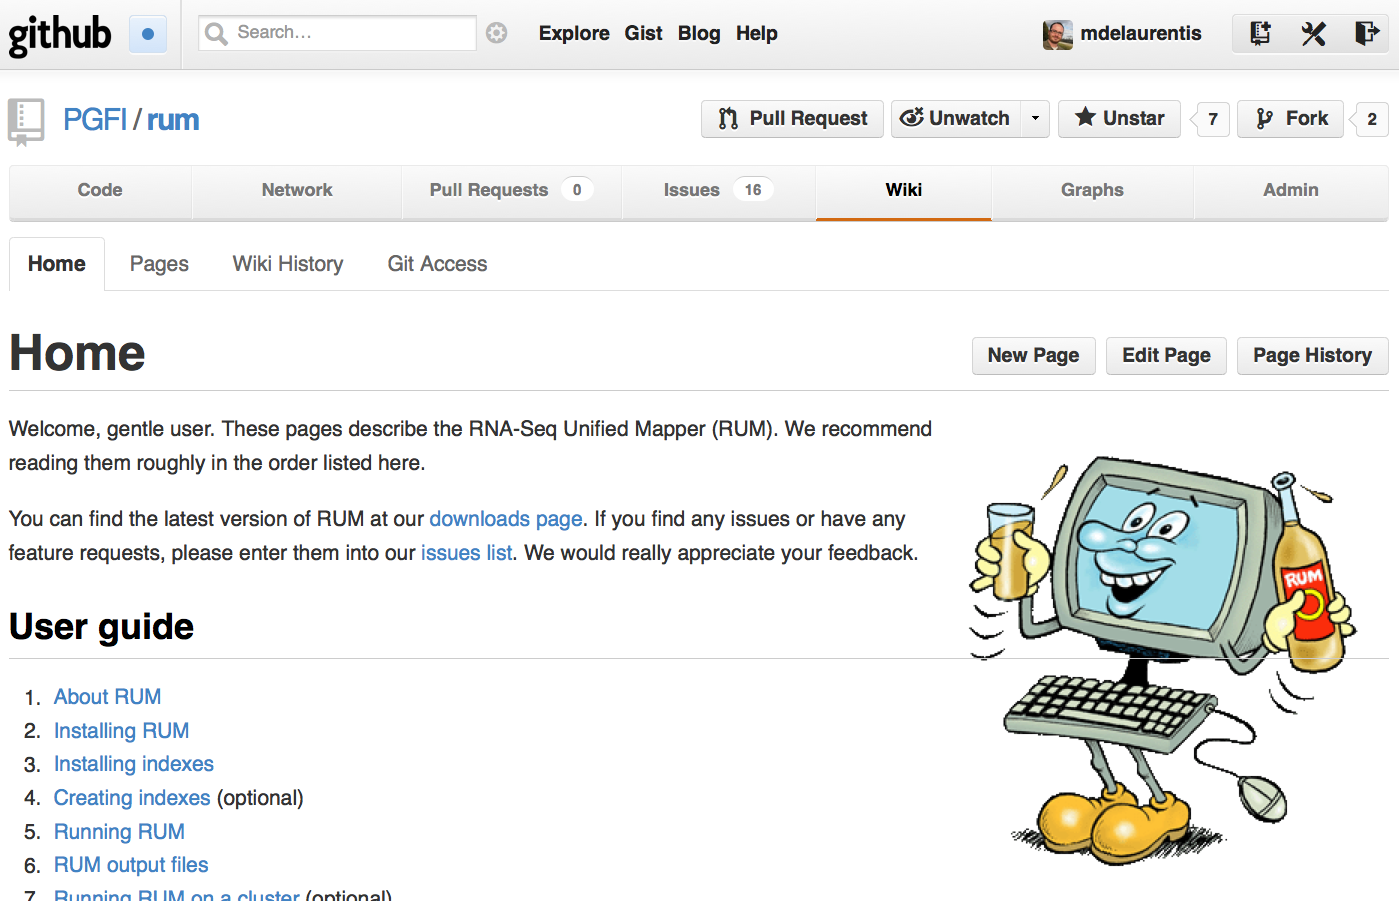
\includegraphics[scale=0.2]{github-wiki.png}
\end{frame}

\subsection{Downloads}

\centering
\begin{frame}{Downloads}
  \url{https://github.com/PGFI/rum/downloads}
  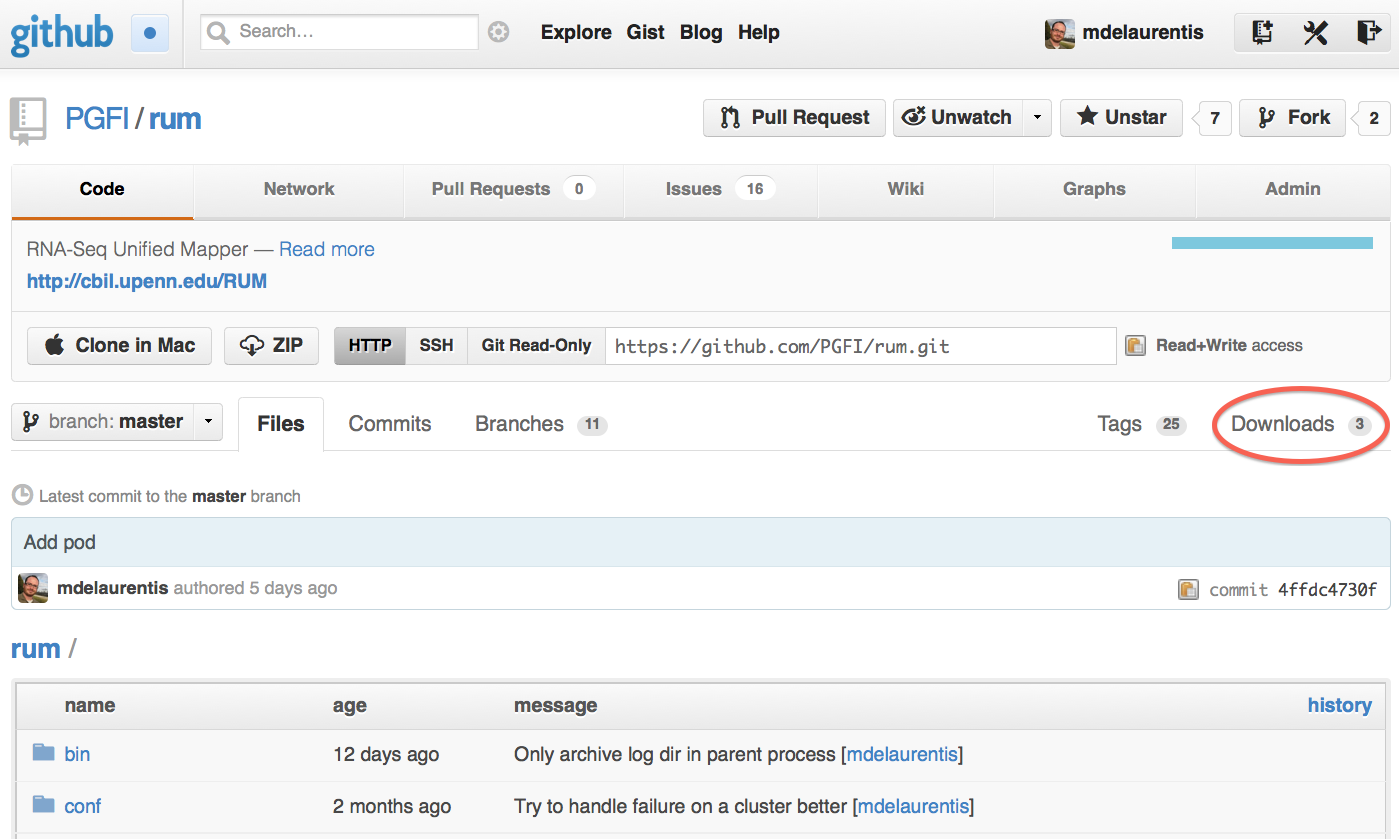
\includegraphics[scale=0.2]{github-main-downloads.png}
\end{frame}

\centering
\begin{frame}{Downloads}
  \url{https://github.com/PGFI/rum/downloads}
  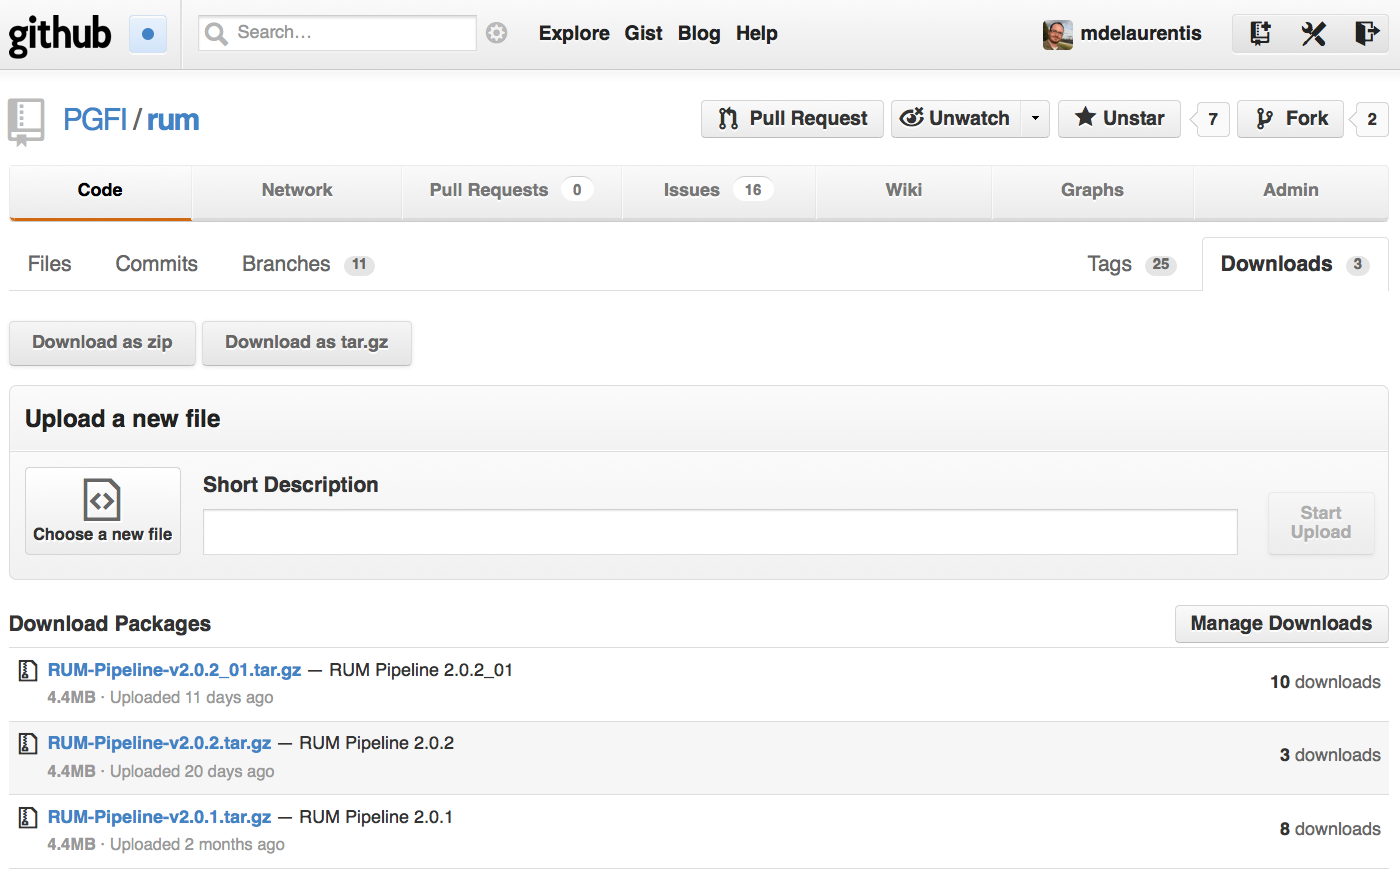
\includegraphics[scale=0.2]{github-downloads.png}
\end{frame}

\subsection{Issues}

\centering
\begin{frame}{Issues}
  \url{https://github.com/PGFI/rum/issues}
  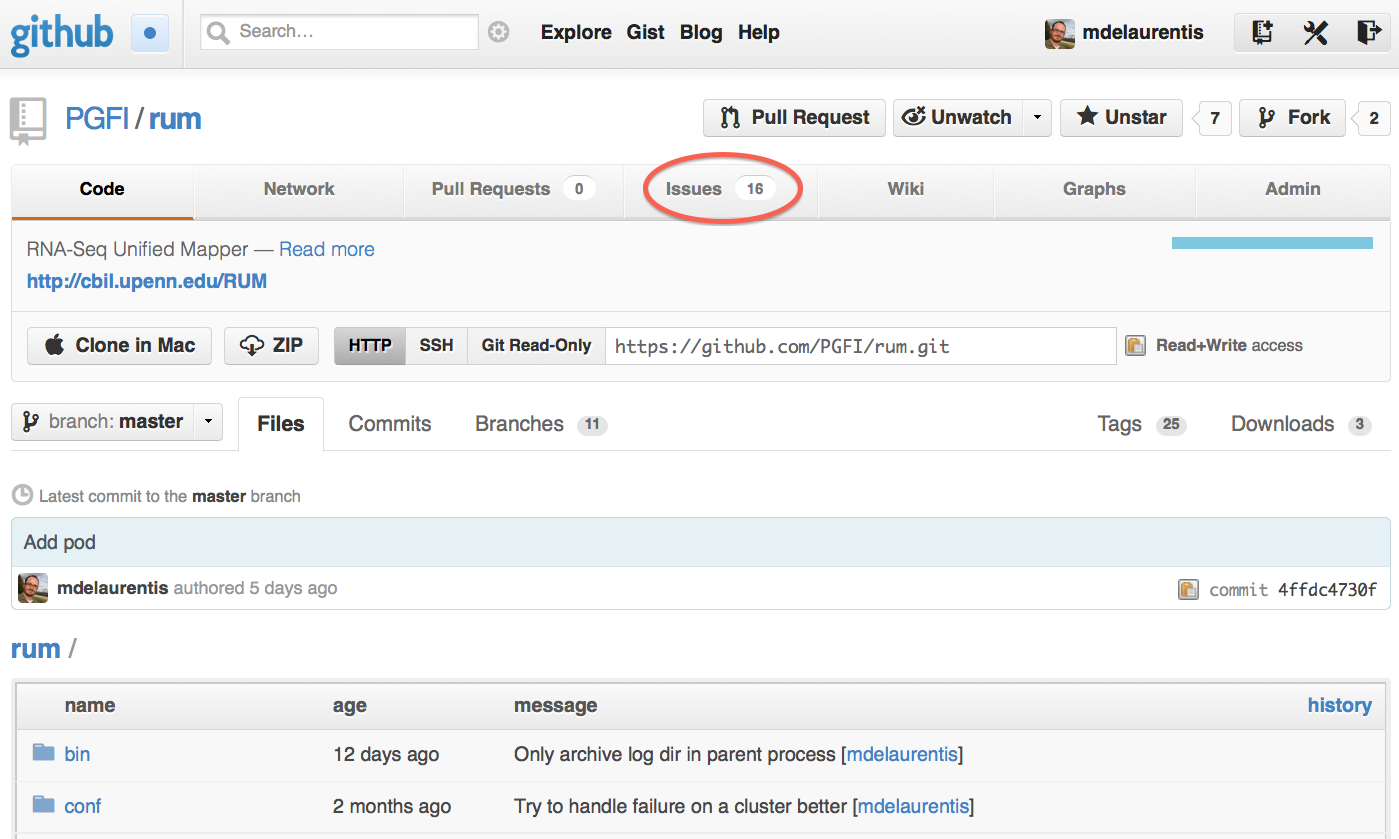
\includegraphics[scale=0.2]{github-main-issues.png}
\end{frame}

\centering
\begin{frame}{Issues}
  \url{https://github.com/PGFI/rum/issues}
  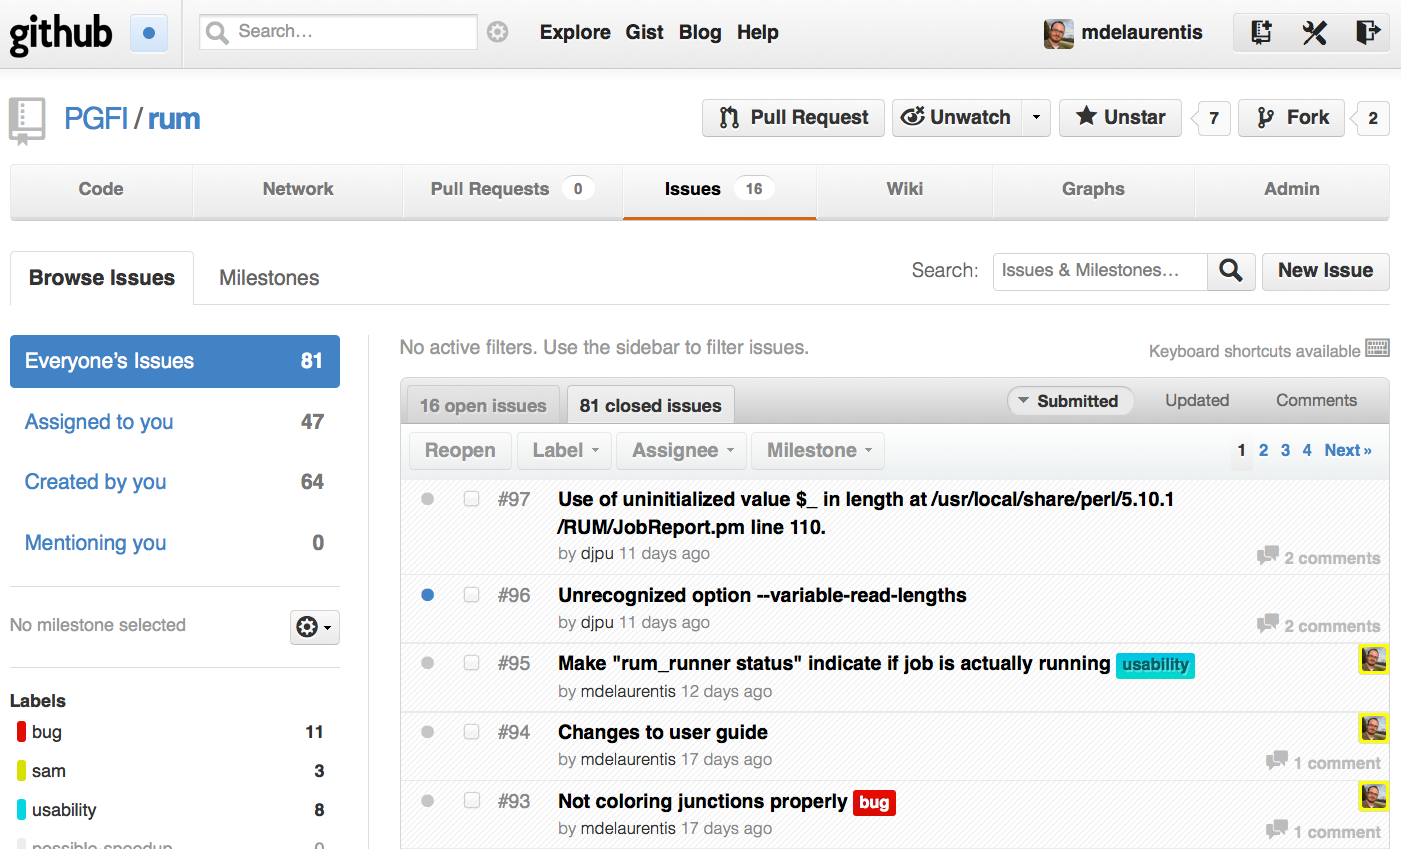
\includegraphics[scale=0.2]{github-issues.png}
\end{frame}

\section{Future direction}

\begin{frame}{Possible future enhancements}
  \begin{itemize}
  \item Use original read names throughout the pipeline
  \item Performance improvements
  \end{itemize}
\end{frame}



\end{document}
